\chapter{Evidence of pair localization in the dynamics of Rydberg spins}\label{ch:experimental-pairs}

In this chapter, we apply the previously derived effective model of pairs to model and interpret experimental results from a Rydberg-based quantum simulator. While the experiment is limited to global control and readout, we make great use of its ability to implement models with different anisotropy and various density (which translates to disorder strength).

We find the pair model to yield  an excellent agreement with the observed behavior explaining both the relaxation dynamics and rescaling thereof~\cite{franzObservationAnisotropyindependentMagnetization2024} as well as the dependence of the steady state magnetization on the strength of the transverse field~\cite{franzEmergentPairLocalization2022}.


\section{Anisotropy-independent relaxation dynamics}\label{sec:universal-dynamics}
In this paper, we utilize the ability of the Rydberg quantum simulator to implement XX, XXZ and Ising models to measure the relaxation of the $x$-magnetization when starting from a fully magnetized state. For disordered Ising models prior work has shown the relaxation to follow a stretched exponential form well-known from spin glasses~\cite{breyStretchedExponentialDecay1993,signolesGlassyDynamicsDisordered2021,schultzenGlassyQuantumDynamics2022,schultzenSemiclassicalSimulationsPredict2022}. It has been conjectured that this type of slow, hierarchical relaxation is a common feature of strongly disordered quantum systems~\cite{haldarSlowDynamicsKohlrausch2023}.

Indeed we find that for all three models the relaxation curves are fitted well by stretched exponentials. Moreover, we also find a scaling law for the characteristic decay time scale which hints at a common origin of the relaxation. This mechanism is explained by the pair model, which yields that for all three models the relaxation is caused essentially by oscillations of the magnetization of pairs. Since each pair has a different oscillation frequency these individual oscillations dephase and thus cause the total magnetization to decay. From the parameter dependence of these pair oscillations, we recover the characteristic timescale for the global magnetization's decay. Thus demonstrating an effective pair localization at least over experimentally relevant timescales.

\newpage
\pdfbookmark[3]{Publication}{universal-dynamics-paper}
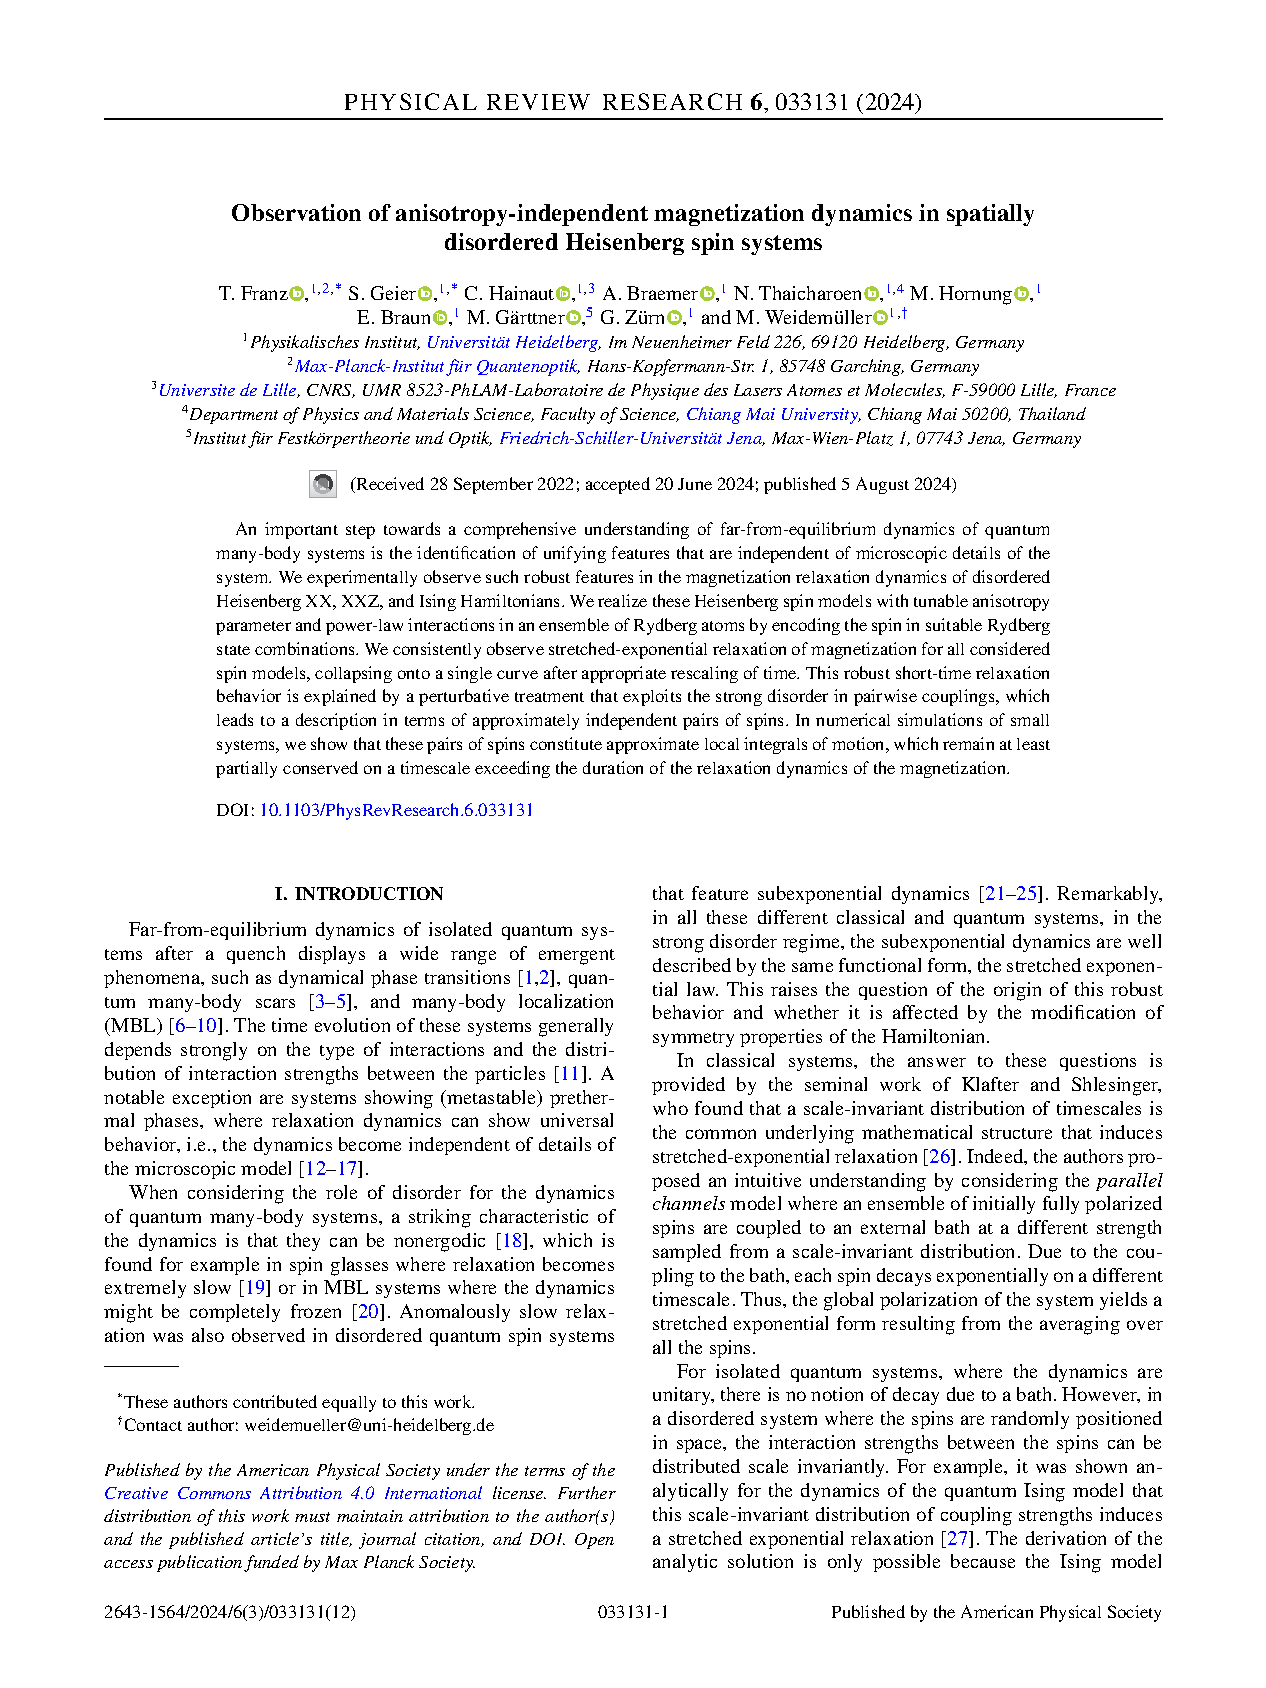
\includepdf[pages=-]{pub-Franz2023-UniversalDynamics}

\section{Emergent pair localization}
Another way of validating the pair model is the comparison of the same system subject different disorder strength. This can be realized in a Rydberg based quantum simulator by tuning the systems density as explained in the background chapter. %TODO reference

In the work below~\cite{franzEmergentPairLocalization2022}, we again use the $x$-magnetization as observable and track its steady-state value with respect to an external magnetic field aligned in $x$-direction as well. We find a clear qualitative difference at weak external field where the strongly disordered system responds much stronger to the field, i.e. the steady-state magnetization grows very fast with increasing field strength. This leads to a sharp cusp-like curve, which we show to be incompatible with a thermal state. However, we find that a pair-based effective model reproduces this feature and can also match the full measurement data closely.
In contrast, for weak disorder, i.e. high density, the behavior of the steady-state magnetization is much different. At weak field, the curve is very round which is reproduced nicely by assuming a thermal state.

Thus, this experiment provides direct evidence for a pair localization transition at least at experimentally relevant timescales. However, it is possible that this is a prethermal regime only and that this signature vanishes at much later times. Testing for this experimentally will of course be very hard if not impossible at all depending on the timescale this final relaxation occurs.

Subsequently (cf. Section \ref{sec:cusp-round-sharp}), we present a simplified alternative to the mean-field model in \cite{franzEmergentPairLocalization2022} that allows for analytical computation of both the thermal and pair localized magnetization curves. While this model is not as quantitative as the mean-field model contained in the publication, it nonetheless reproduces the curves qualitatively and highlights the physical origin of the behavior at weak field more directly.

\newpage
\pdfbookmark[3]{Publication}{cusp-paper}
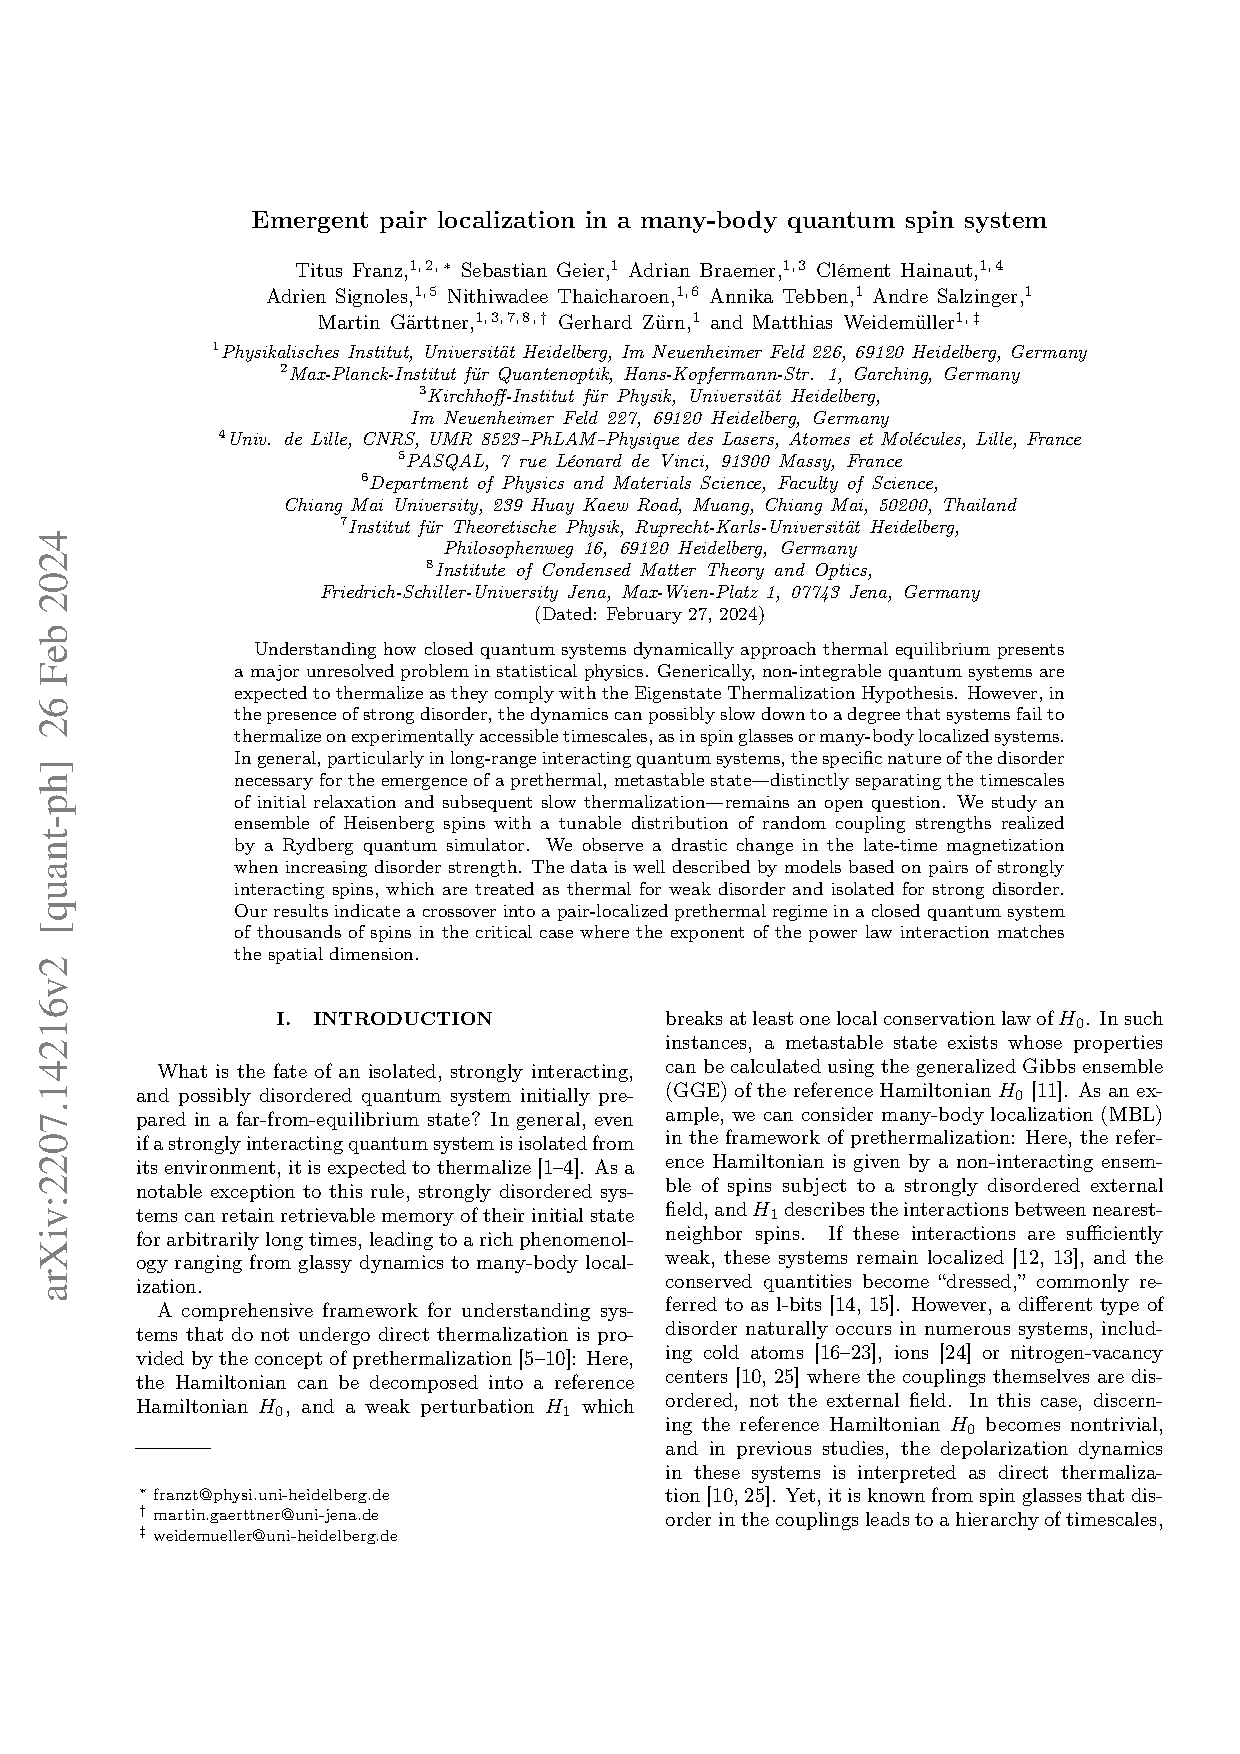
\includepdf[pages=-]{pub-Franz2022-Cusp}

\subsection{Simple physical picture}\label{sec:cusp-round-sharp}
To derive the qualitative behavior of the steady-state magnetization $\braket[1]{M(\Omega)}$ with respect to external field $\Omega$, we use a simple two-component model where each spin is either fully polarized or fully demagnetized. We assume that a spin's final state depends solely on the ratio of the strongest coupling $J$ towards another spin and the strength of the external field $\Omega$. If the field dominates, i.e. $|\Omega| > J$, the spin stays polarized as it is locked by the field. Conversely, if the coupling dominates, i.e. $|\Omega| < J$, then the interactions lead to depolarization and the spin loses its magnetization. Thus in this simplified model, the only quantity determining the steady-state magnetization is the distribution of relevant couplings $P(J)$:
\begin{equation}\label{eq:Cusp-simple-model-magnetization}
	\braket[1]{M(\Omega)} = \frac{1}{2}\int_0^{|\Omega|}\!\mathrm{d}J P(J)
\end{equation}

%TODO rephrase and use P_NN(J) as well
In the regime of weak disorder, it only natural to assume that the strongest relevant coupling for a spin is given by the coupling to its nearest neighbor. In contrast for strong disorder where we assume the pair model to describe the dynamics, the nearest neighbor coupling usually is not the relevant coupling! Instead, we need to consider the distribution of pair couplings $P_{pair}(J)$, i.e. the distribution of couplings that are shared by spins of the same pair.

To compute these coupling distributions analytically, we go to the limit of vanishing blockade radius, i.e. $r_b\rightarrow 0$, and assume that spins are distributed randomly with uniform density $\rho$ in $d$ dimensional space. Fixing some spin, this gives us for the number of spins in spherical shell of size $r$ and width $\mathrm{d}r$
\begin{equation}\label{eq:uniform-spin-distribution}
	w_u(r)\mathrm{d}r = d \rho \Omega_d r^{d-1}\mathrm{d}r = d\lambda (\lambda r)^{d-1}\mathrm{d}r
\end{equation}
where $\Omega_d = \frac{\pi^{d/2}}{\Gamma(n/2+1)}$ is the volume of a $d$-dimensional unit sphere and $\lambda^d = \rho \Omega_d$ is akin to the inverse mean distance between spins. We use this setup to compute both the distribution of nearest neighbor coupling $P_{NN}(J)$ and the distribution of pair couplings $P_{pair}(J)$ in the following sections.

\subsubsection{Nearest-neighbor coupling distribution $P_{NN}(J)$}

The distribution of the nearest neighbor couplings can be found using a simple ansatz~\cite{chandrasekharStochasticProblemsPhysics1943}. Consider some fixed spin and the density of spin $w(r)$ at distance $r$. Then the probability $P_{NN}(r)$ of finding the nearest neighbor of that fixed spin at distance $r$ should be proportional to both the probability of having a spin in that distance and the probability of having no closer neighbor. This gives us the following integral-equation 
\begin{align}\label{eq:nn-integral-eq}
	P_{NN}(r) = w(r)*\left(1-\int_0^r \mathrm{d}r' P_{NN}(r')\right)
\end{align}
which can be solved straight-forwardly by noting that it has the form $f' = -w f$ and using separation of variables. The solution reads:

\begin{equation}\label{eq:nn-distribution}
	P_{NN}(r) = w(r)\exp\left(-\int_0^r \!\mathrm{d}r' w(r')\right)\quad.
\end{equation}

Plugging in the distance distribution for uniform spin density $w_u(r)$ (cf. Eq.~\ref{eq:uniform-spin-distribution}) gives us a so-called Weibull distribution:

\begin{align}\label{eq:weibull-distribution}
	P_{NN}(r) = d \lambda^d r^{d-1} \exp(- \lambda^d r^d)
\end{align}

Finally, changing variables\footnote{Note, the change of variables also needs to transform the measure, i.e. we transform $P(r)\mathrm{d}r \!\rightarrow\! P(J)\mathrm{d}J$} from distance $r$ to coupling $J=r^{-\alpha}$ yields the sought-after distribution of nearest-neighbor couplings
%
%\begin{align}
%	r &= J^{-\frac{1}{\alpha}}\\
%	\mathrm{d}r &= \frac{-1}{\alpha}J^{-\frac{1}{\alpha}-1}\mathrm{d}J
%\end{align}
%
%The sign of the Jacobi-Determinant is to be neglect and we obtain:
%
\begin{equation}\label{eq:P-NN-J}
	P_{NN}(J) = \beta\lambda^d J^{-\beta-1} \exp\left(-\lambda^d J^{-\beta}\right)
\end{equation}
where $\beta=\frac{d}{\alpha}$.

\subsubsection{Distribution of pair couplings $P_{pair}(J)$}
%TODO clear up difference pair <-> NN?
We can derive the distribution of pair lengths in a similar fashion to Eq.~\ref{eq:nn-integral-eq}. The key insight about the difference between a nearest neighbor and the partner of a pair in the RSRG sense is that the two partners of the pair are in some sense each other's partner. In contrast the "nearest neighbor" property does not need to be reflexive. Denoting the pair coupling distribution as $P_{pair}(J)$, we write down the respective integral equation, which is very similar to Eq.~\ref{eq:nn-integral-eq}, except that the second factor gets squared because \emph{both spins} may not be part of a smaller pair:

\begin{align}\label{eq:pair-integral-eq}
	P_{pair}(r) = w(r)*\left(1-\int_0^r \mathrm{d}r' P_{pair}(r')\right)^2
\end{align}

%We can solve this equation rather easily by separation of variables (easy once you know what to do that is...):
%
%\begin{align}
%	w_P(r) = w(r)*\left(1-\int_0^r \mathrm{d}r' w_P(r')\right)^2\\
%	\Leftrightarrow \int_0^R \mathrm{d}r \frac{w_P(r)}{\left(1-\int_0^r \mathrm{d}r' w_P(r')\right)^2} = \int_0^R \mathrm{d}r w(r)\\
%	\Leftrightarrow \frac{1}{1-\int_0^R \mathrm{d}r' w_P(r')} - 1 = \int_0^R \mathrm{d}r w(r)\\
%	\Leftrightarrow \int_0^R \mathrm{d}r' w_P(r') = 1- \frac{1}{1 + \int_0^R \mathrm{d}rw(r)}\\
%	\Leftrightarrow w_P(R) = \frac{w(R)}{\left(1 + \int_0^R \mathrm{d}rw(r)\right)^2}\\
%	\Rightarrow w_P(r) = \frac{d\mathrm{vol}_d(1)r^{d-1}}{\left(1 + \mathrm{vol}_d(1)r^d\right)^2} = \frac{d}{\lambda} \frac{\left(\frac{r}{\lambda}\right)^{d-1}}{\left( 1+\left(\frac{r}{\lambda}\right)^d\right)^2}
%\end{align}

This equation can be solved in the same way as Eq.~\ref{eq:nn-integral-eq} and yields
\footnote{Eq.~\ref{eq:pair-distribution} was derived by a different method for $d=3$ by former Master student Péter Kaposvári in his Master thesis~\cite{peterMasterThesis}.}:

\begin{align}\label{eq:pair-distribution}
	P_{pair}(r) = \frac{w(r)}{\left(1+\int_0^r\!\mathrm{d}r' w(r')\right)^2}
\end{align}

Employing the distance distribution for uniform spin density $w_u(r)$ (cf. Eq.~\ref{eq:uniform-spin-distribution}) again gives us that the pair distances follow a \emph{log-logistic distribution} for spins of uniform density:

\begin{equation}\label{eq:log-logistic-distribution}
	P_{pair}(r) = \frac{d\lambda^d r^{d-1}}{\left(1 + \lambda^d r^d\right)^2 }
\end{equation}

Changing to distance $r$ to coupling $J=r^{-\alpha}$ yields:

\begin{equation}\label{eq:P-pair-J}
	P_{pair}(J) = \frac{\beta\lambda^d J^{-\beta-1}}{\left(1+\lambda^{d}J^{-\beta}\right)^2}
\end{equation}

\subsubsection{Analytical steady-state magnetization}

\FIXME{maybe integrate the curves from CUSP paper for better comparison?}

\begin{figure}[htb]
	\centering
%	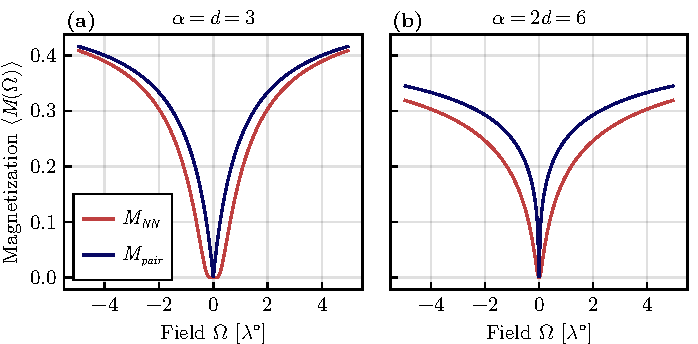
\includegraphics{part1/analytical_cusp}
	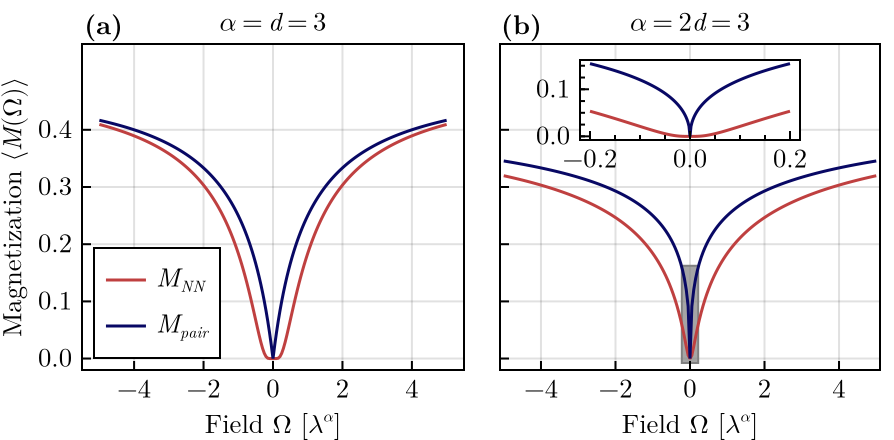
\includegraphics{part1/analytical_cusp_inset}
	\caption{Steady-state magnetization curves of the simple two-component model using the same color scheme as Fig.~2 (d) and (e) of \cite{franzEmergentPairLocalization2022}. Parameters, $\alpha$ and $d$ correspond to (a) Fig.~2 (b) Fig.~4.
	The inset show a zoom around $\Omega=0$ to highlight the qualitative difference between the curves.
	% TODO
	}
	\label{fig:analytical-cusp}
\end{figure}

Having derived both the distribution of nearest-neighbor coupling $P_{NN}(J)$ (Eq.~\ref{eq:P-NN-J}) and pair coupling distribution $P_{pair}(J)$ (Eq.~\ref{eq:P-pair-J}), we can compute the steady-state magnetization of our simple model by using Eq.~\ref{eq:Cusp-simple-model-magnetization}:
\begin{align}
	M_{NN}(\Omega) &= \frac{1}{2}\int_0^{|\Omega|}\!\mathrm{d}J\ P_{NN}(J) = \frac{1}{2}\exp(-\lambda^d |\Omega|^{-\beta})\\
	M_{pair}(\Omega) &= \frac{1}{2}\int_0^{|\Omega|}\!\mathrm{d}J\ P_{pair}(J) = \frac{1}{2+2\lambda^{d}|\Omega|^{-\beta}}
\end{align}

The resulting curves (cf. Fig.~\ref{fig:analytical-cusp}) show the same qualitative features as their counterparts in \cite{franzEmergentPairLocalization2022}. Thus, this simple model gives us insight in the key mechanism behind the qualitative change of the steady-state magnetization behavior: At weak field $|\Omega|\ll 1$, the magnetization is determined by the weakest interactions $J<|\Omega|\ll 1$ which stem from long distances $r \gg 1$. For nearest neighbors, the distribution of distances is suppressed exponentially $\propto \exp(-r^d)$ (cf. Eq.~\ref{eq:weibull-distribution}), which creates the very smooth, round shape at weak field. Conversely, if the relevant lengths are given by the pairing procedure, the exponential suppression is weakened to an algebraic decay $\propto r^{-d-1}$. Intuitively, this is because while with increasing distance $r$ the number of potential partners increases, it also becomes less likely that they are still available. This competition then leads to a much slower decay of the relevant lengths.

\subsubsection{Discussion}

\begin{figure}[htb]
	\centering
	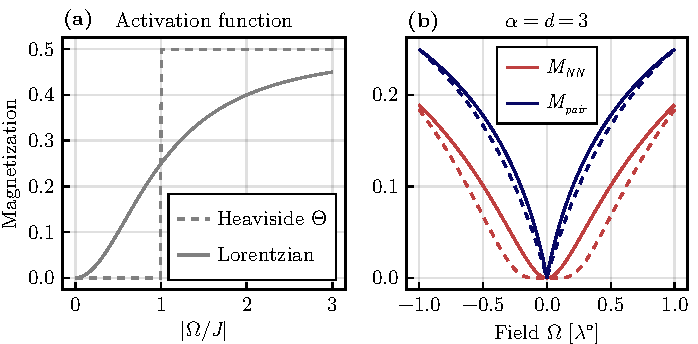
\includegraphics{part1/analytical_cusp_comparison_lorentz}
	\caption{Comparison of the two-component model (dashed lines) with another model where the constituents' magnetization is given by a Lorentzian (solid lines). (a) steady-state magnetization of the constituent. (b) predictions of both model for $\alpha=d=3$ [same parameters as Fig.~\ref{fig:analytical-cusp}(a)].
	}
	\label{fig:analytical-cusp-comparison-lorentz}
\end{figure}

The two-component model developed here is of course much simpler than the mean-field used in \cite{franzEmergentPairLocalization2022} but we argue that it captures the essential physics nonetheless. The two main conceptual differences are: The mean field model considers the magnetization response of pairs, which is a Lorentzian [cf. Eq.~(C3)], and additionally solves the equations self-consistently to capture the influence of a pairs magnetization on other pairs in the vicinity. The latter is responsible an the asymmetry of the ensemble's magnetization because the induced magnetization enhances (weakens) the effective magnetic field if external field and initial polarization are aligned (anti-aligned) to each other. This essentially introduces a small scaling factor for positive field for the field relative to negative values but does not change the qualitative behavior at weak field (cf. Fig.~5 of \cite{franzEmergentPairLocalization2022}). 

To check the effect of the Lorentzian magnetization function, we can generalize the two-component model slightly at the cost of it being no longer analytically solvable. We replace the idea of single spins that are either locked by the field or dominated by interaction by more general constituents that just follow some activation function, i.e. a function $m(\omega)$ that gives the resulting magnetization for a given ratio $\omega=\Omega/J$ of field strength $\Omega$ and relevant coupling $J$. Then the total steady-state magnetization reads

\begin{equation}\label{eq:generalized-two-component-model}
	\braket[1]{M(\Omega)} = \frac{1}{2}\int_0^{\infty}\!\mathrm{d}J P(J)m\left(\frac{\Omega}{J}\right)
\end{equation}
and the two-component model is recovered with $m(\omega)=\Theta(\omega - 1)$ where $\Theta$ denotes the Heaviside function. For a pair the magnetization follows a Lorentzian curve (cf. Eq.~(C3) of \cite{franzEmergentPairLocalization2022}), which in this notation is given by $m_L(\omega) = \frac{\omega^2}{1+\omega^2}$. As Fig.~\ref{fig:analytical-cusp-comparison-lorentz} shows, this does not alter the qualitative behavior at weak external field. Thus we conclude that the observed qualitative change of the steady-state magnetization stems from a fundamental change in character of the distribution of relevant couplings.

%Behavior around 0: Both non-analytic. $P_{NN}$ very round, all derivatives vanish. $P_{pair}$ non-analytic for $\beta\leq1$ i.e. $d \leq \alpha$.
%A few remarks:
%For $J\rightarrow 0$ this gives the limits:
%
%\begin{equation}
%	\lim_{J\rightarrow0} w_P(J) = \lim_{J\rightarrow0} \beta\lambda^{-d} J^{\beta-1} =\begin{cases}0 & d>\alpha\\ \beta\lambda^{-d} & d=\alpha\\ \infty & d<\alpha\end{cases}
%\end{equation}
%
%The Cusp thus acquires the form:
%
%\begin{equation}
%	\int_0^h\! \mathrm{d}J\ w_P(J) = \left. \frac{1}{1+\lambda^{d}J^{-\beta}}\right|_{0}^h = \frac{1}{1+\lambda^{d}h^{-\beta}}
%\end{equation}
%
%Note: For $\alpha > d$ this predicted cusp gets ultra sharp as the first derivative diverges at $0$!


%\begin{figure}[htb]
%	\centering
%	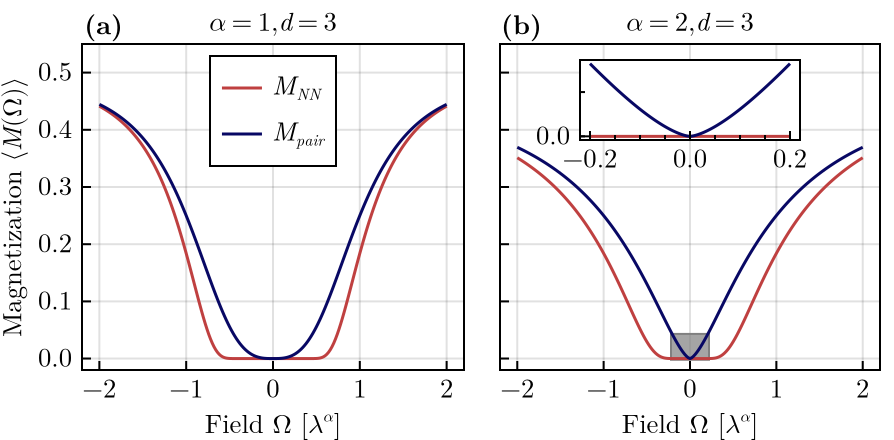
\includegraphics{part1/analytical_cusp_alpha_small}
%	\caption{Steady-state magnetization curves of the simple two-component model using the same color scheme as Fig.~2 (d) and (e) of \cite{franzEmergentPairLocalization2022}. Shown are two examples where $\alpha < d$.
%	}
%	\label{fig:analytical-cusp-alpha-small}
%\end{figure}

